\subsection{Live Programming with Incomplete Expressions}

The process of writing new program fragments includes many states in which the
program under construction is, by definition, incomplete.
%
It is natural for a programmer to ``jump back and forth'' between different
places in the program, iteratively and alternately developing the missing
pieces.
%
The primary benefit of our approach is that such programs can be evaluated in
order to provide useful feedback during this editing workflow.

% !TEX root = hazelnut-dynamics.tex

\begin{figure}[t]
\begin{subfigure}[t]{\textwidth}
\centering
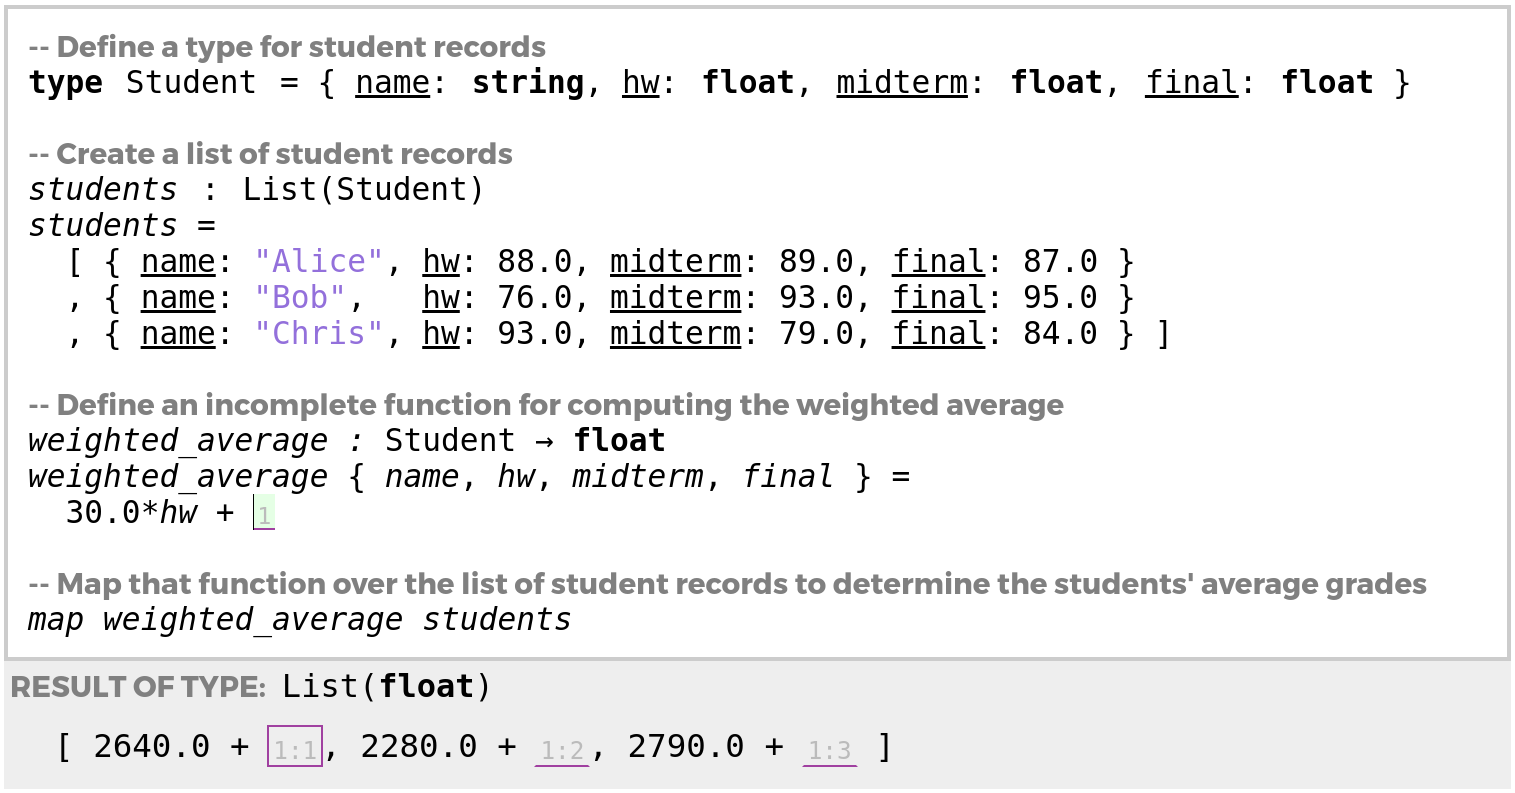
\includegraphics[width=0.8\textwidth,interpolate=false]{images/grades-cell-mockup.png}
\vspace{-3px}
\caption{Evaluating an incomplete functional program past the first hole}
\label{fig:grades-cell-mockup}
\end{subfigure}

\vspace{10px}

\begin{subfigure}[t]{\textwidth}
\centering
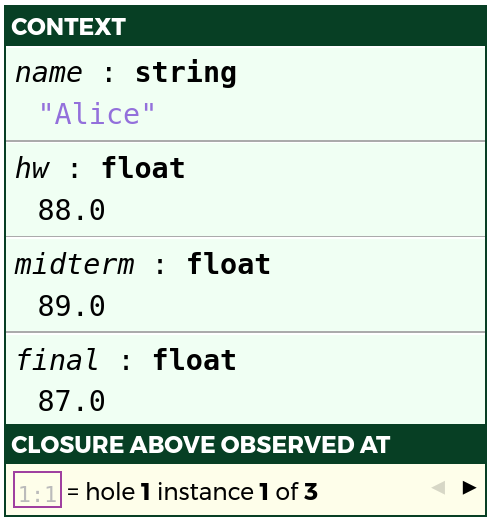
\includegraphics[width=0.29\textwidth,interpolate=false,valign=c]{images/grades-sidebar-1.png}
~${}^\blacktriangleright$
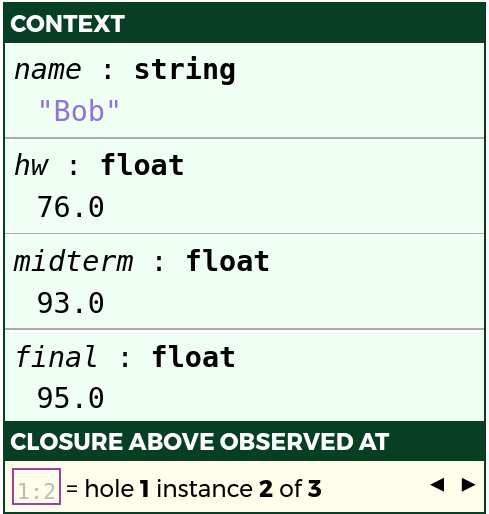
\includegraphics[width=0.29\textwidth,interpolate=false,valign=c]{images/grades-sidebar-2.png}
~${}^\blacktriangleright$
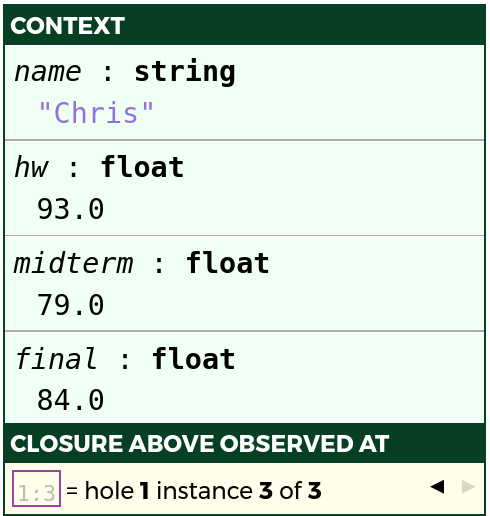
\includegraphics[width=0.29\textwidth,interpolate=false,valign=c]{images/grades-sidebar-3.png}
\caption{The live context inspector communicates relevant static \emph{and} dynamic information about variables in scope.}
\label{fig:grades-sidebar}
\end{subfigure}
% %% TODO once the code above is removed, scale up the screenshots
% 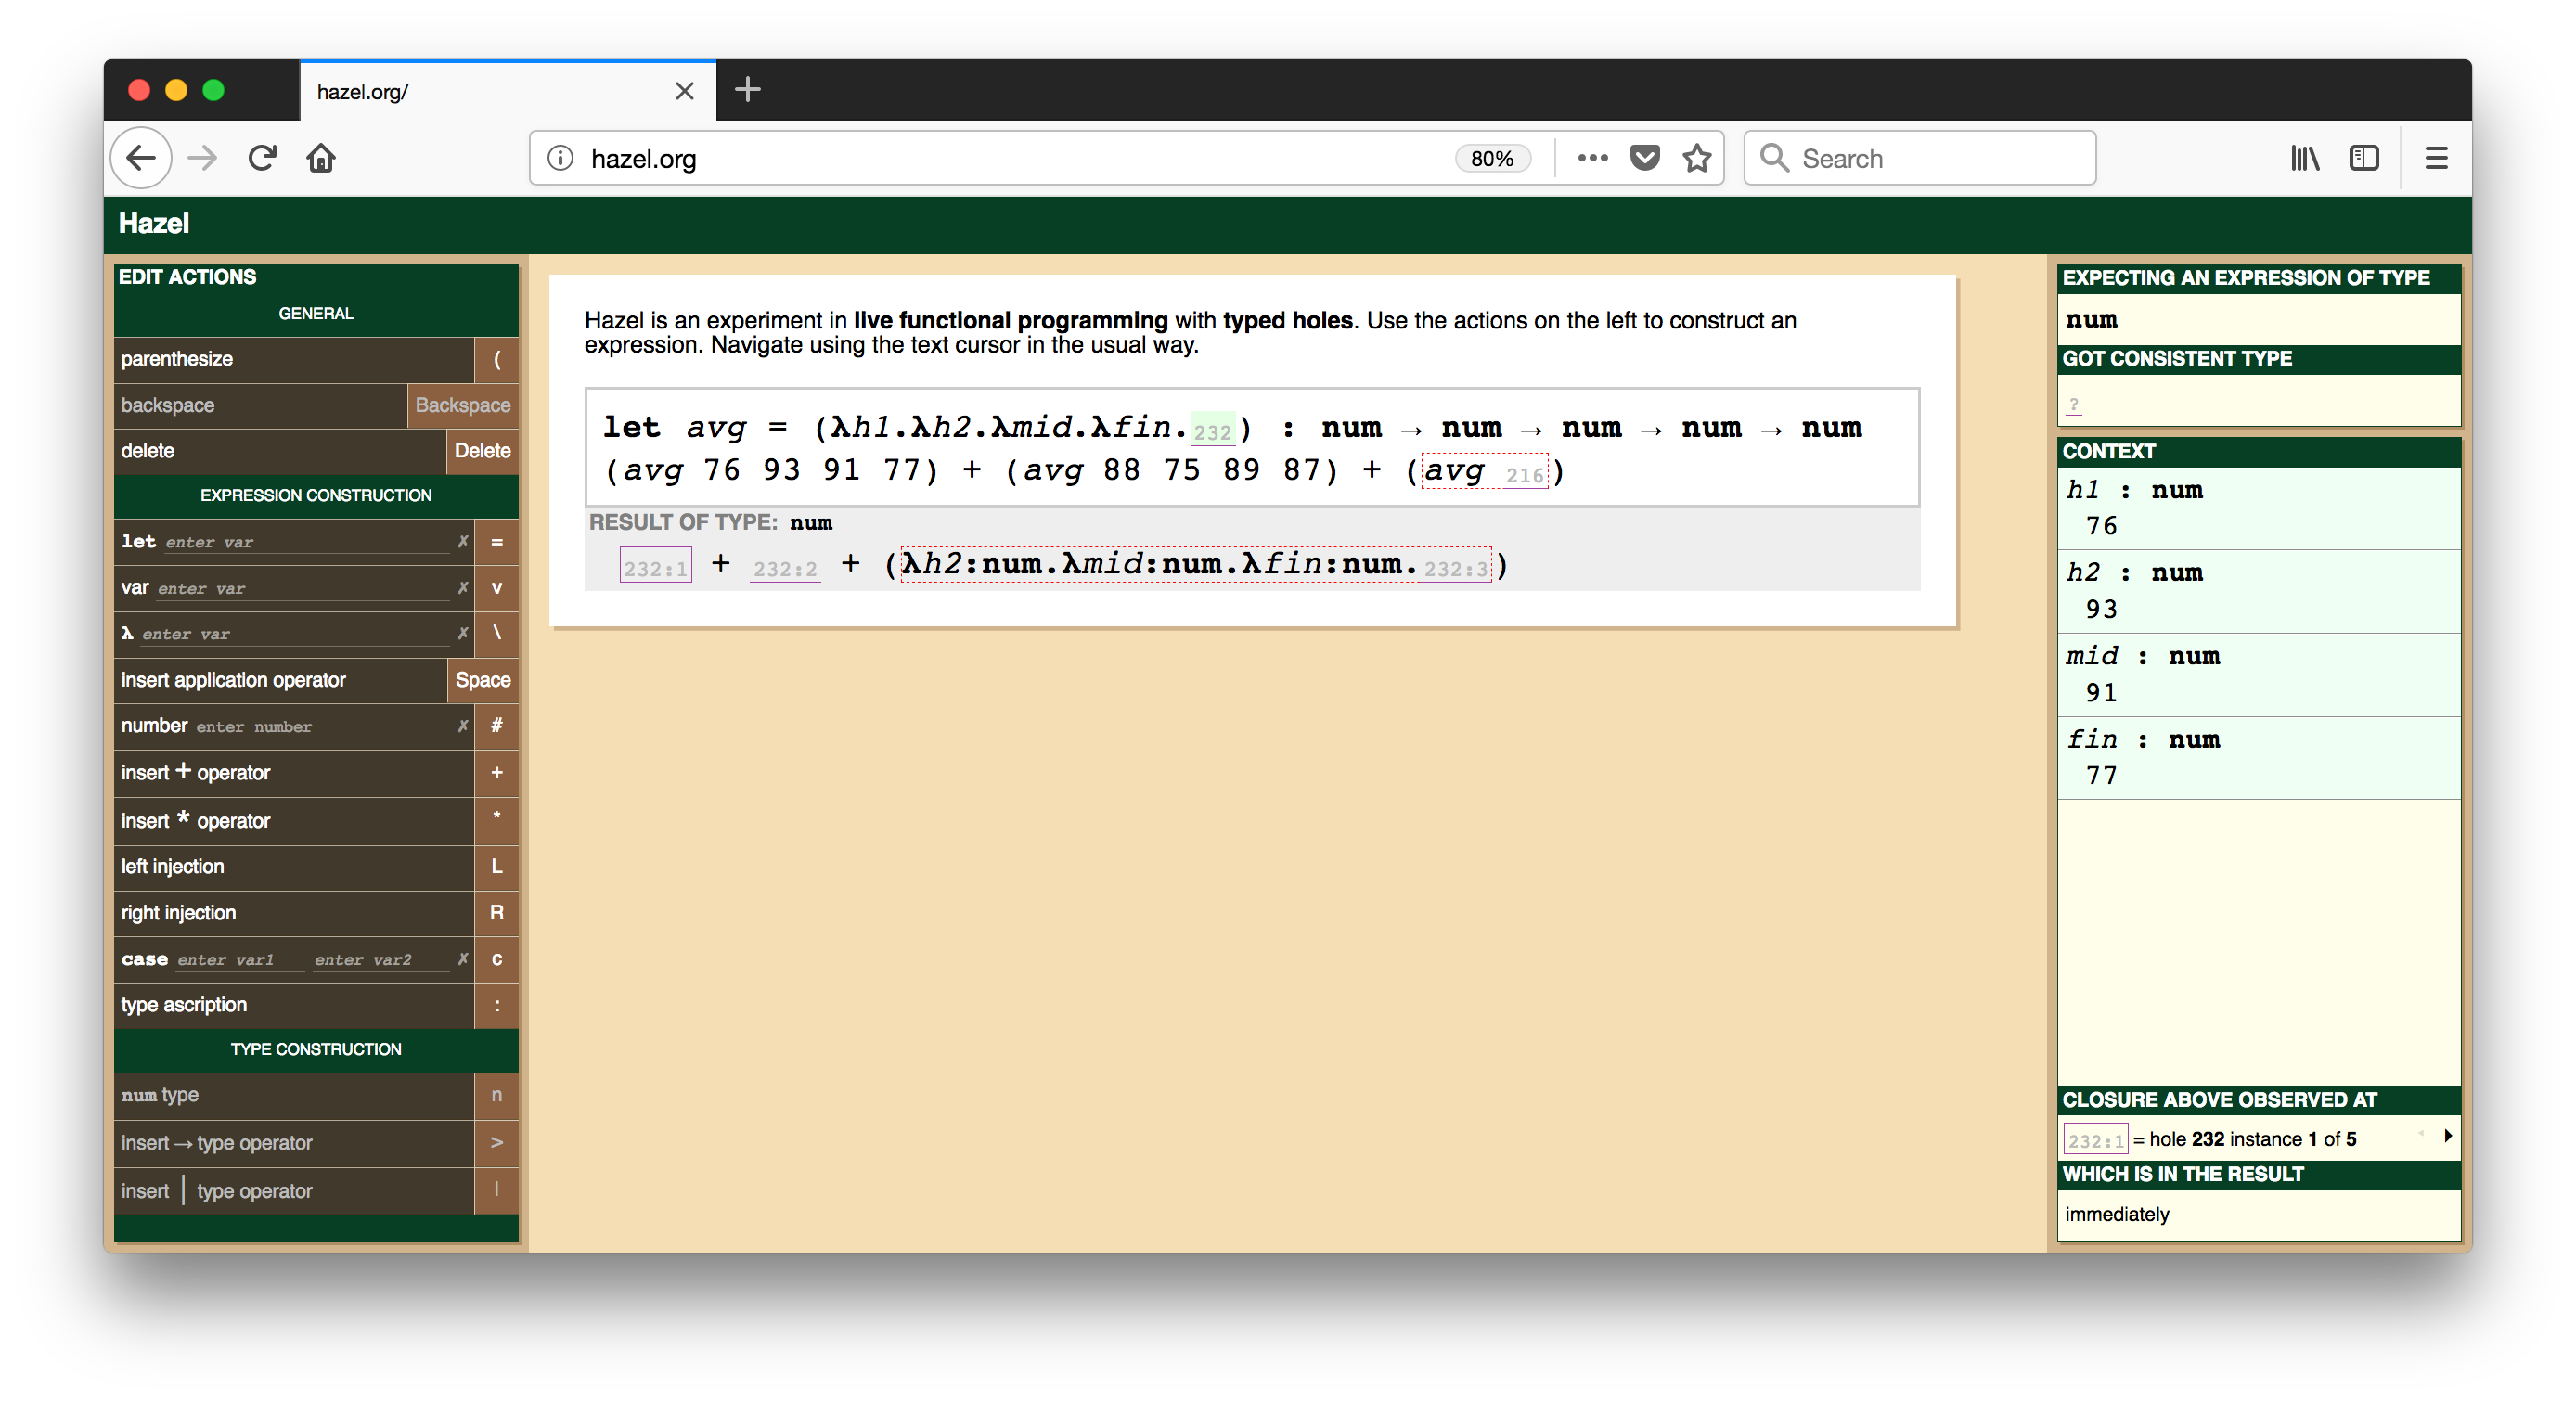
\includegraphics[scale=0.20]{images/hazel-placeholder-0.png}

% \rkc{Draw arrows and captions on the top figure to show how to get
% to the bottom figure.
% ser navigates to hole a, types + to create a plus, types * to create a
% multiplication, types \#10 to create 10, types vh1 to create variable use.}

% 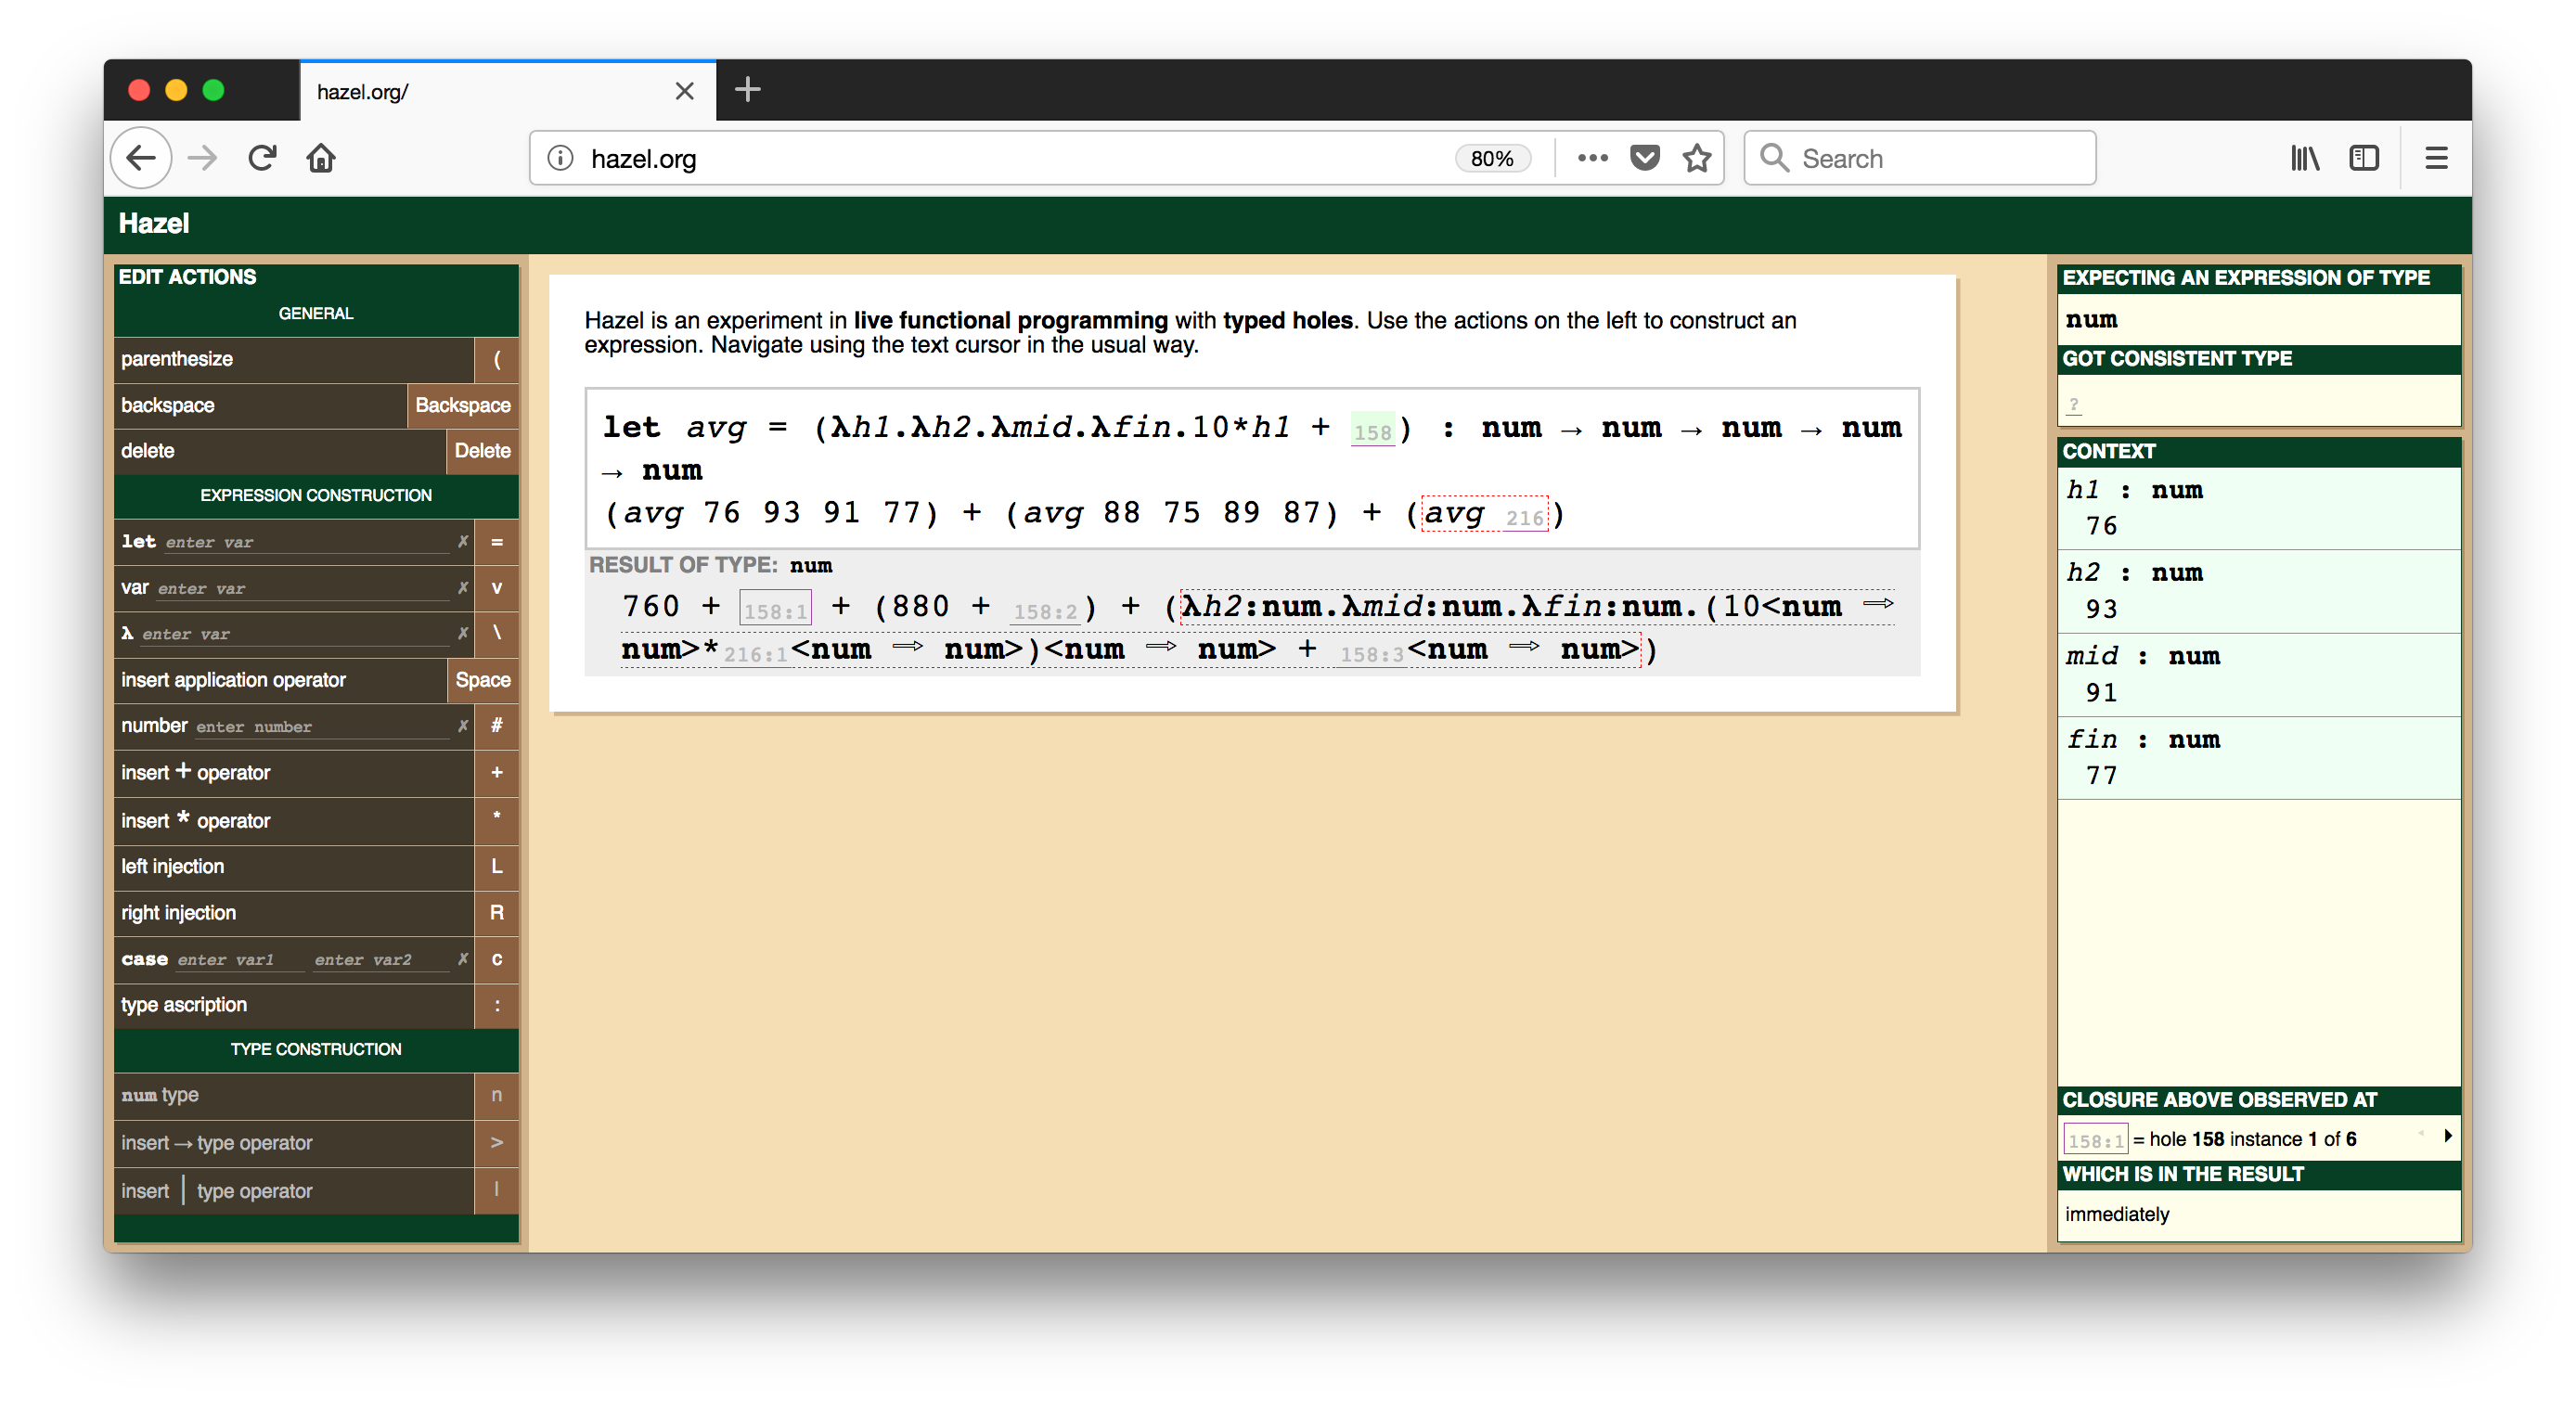
\includegraphics[scale=0.20]{images/hazel-placeholder-1a.png}
\vspace{3px}

\caption{Example 1: Grades}
\label{fig:grades-example}
\vspace{-5px}
\end{figure}


\overviewExample{1a}{Computing Weighted Averages}
%
Consider a teacher who is in the midst of developing a \Hazel{} notebook
(depicted at the top of \autoref{fig:grades-example}) to compute final student
grades at the end of a term.
%
At the top of the program, the teacher defines a
record type, \li{student_data}, for each student's course data.
%
In our simplified example, this includes the student's name, of type
\li{string}, and five grades, each of type \li{float}.

The teacher begins writing a \li{weighted_average} function that will
compute a weighted average, of type \li{float}, for each \li{student_data}
record.
%
The body of \li{weighted_average} is not yet written---marked with the
\emph{empty hole} on line \rkc{XXX}---but the teacher jumps ahead to map the
function over the \li{grades} list on line \rkc{XXX}.
%
\Hazel{} evaluates this incomplete program, showing its
\emph{indeterminate} result in \emph{results panel} just below the
program in the center of the window (\autoref{fig:grades-example});
this value is a list whose length is the same as
\li{grades}, where each element is the (indeterminate) result of evaluating the
hole expression inside \li{weighted_average}.
%
\rkc{The editor shows the first three elements of a result list, by default; the
... can be clicked and expanded to see additional elements.}

Notice that the hole expression on line \rkc{XXX} is assigned a unique static
identifier (\ie{}~\li{a}) and that the indeterminate results it produces are
assigned corresponding unique dynamic identifiers (\ie{}~\li{a.1}, \li{a.2},
etc.).
%
In contrast, the typical ad-hoc approach to simulating hole expressions, namely,
using placeholder expressions like \li{raise "Not yet implemented."}, would halt
the program as soon it is evaluated (in this case, inside the definition of
\li{List.map} when the function is applied to the first element of \li{grades}.
%
By ``evaluating around'' the hole in \HazelnutLive{}, the programmer can at
least see that the resulting expression does indeed evaluate to a list with the
correct number of (indeterminate) values.

Now the teacher returns to \li{weighted_average} to work on the missing
expression, with the goal of computing a weighted sum of each of a student's
grades.
%
The teacher performs several \Hazel{} edit actions (each of which is a single
keystroke, a shortcut to selecting one of the edit tools from the left panel,
followed by a tool-specific argument terminated with the Enter key):
%
navigating the cursor to hole \li{a} and typing \li{+}, which creates a
sum expression \li{??_b + ??_c} with the cursor placed, by default, under
left operand (the hole labeled \li{b});
%
typing \li{*} to create a multiplication expression \li{??_d * ??_e + ??_c},
with the cursor place under hole \li{d};
%
typing \li{\#10} to enter a numeric scaling factor, which then moves
the cursor to the second operand, hole \li{e}; and
%
typing \li{vg.hw1} to use the \li{hw1} field of the function argument
as the right operand of the multiplication.
%
The resulting partial expression, \li{(10.0 *. g.hw1) +. ??_b}---shown
in the screenshot in the bottom half of \autoref{fig:grades-example}---marks the
first of five weighted summands in the eventual finished \li{weighted_average}
calculation.

Each \Hazel{} edit action transforms an incomplete but well-formed and
well-typed program into another such program, and, thus, \Hazel{} immediately
runs the program after each edit.
%
After the above edit sequence, \Hazel{} display the updated list of
indeterminate expressions \li{[760.0 + ??_b.1, 880.0 + ??_b.2, ...]}.
%
Right away, the teacher recognizes that the values are too large; they should be
at most \li{100.0}.
%
The teacher realizes that representing percentage points as \li{float}s requires
that the constant on line \rkc{XXX} ought to be \li{0.10} instead.
%
Because of this live feedback, the teacher corrects this error right away and
avoids making similar programming errors in the rest of the calculation.
%
The teacher continues to build the rest of the arithmetic expression until it is
complete (there are no longer any expression holes), and the result of
immediately running the finished program shows that each of values in the final
result list is in the range \li{0.0} to \li{100.0}.

\begin{figure}[t]

\rkc{Move all this code into the mockup screenshots below.}

\lstset{basicstyle=\scriptsize\ttfamily}
\begin{lstlisting}
type grade_cutoffs =
  { a: float, b: float, c: float, d: float, f: float };

let cutoffs =
  { a = ??_a, b = ??_b, c = ??_c, d = ??_d, f = ??_f };

let letter_grade(n: weighted_average) =
  if n >= cutoffs.a then "A" else
  if n >= cutoffs.b then "B" else
  if n >= cutoffs.c then "C" else
  if n >= cutoffs.d then "D" else
  if n >= cutoffs.f then "F" else "Incomplete";

let sorted_weighted_averages = List.sort weighted_averages;

let letter_grades = List.map letter_grade sorted_weighted_averages;

let compute_distribution(list: list(float)) =
  let n = List.length letter_grades in
  List.map
    (\x -> (x, showPercentage (List.length (List.filter ((==) x) list)) /. n))
    ["A","B","C","D","F","Incomplete"];

let distribution = compute_distribution(letter_grades);
\end{lstlisting}
%% restore settings from main.tex
\lstset{basicstyle=\footnotesize\ttfamily}

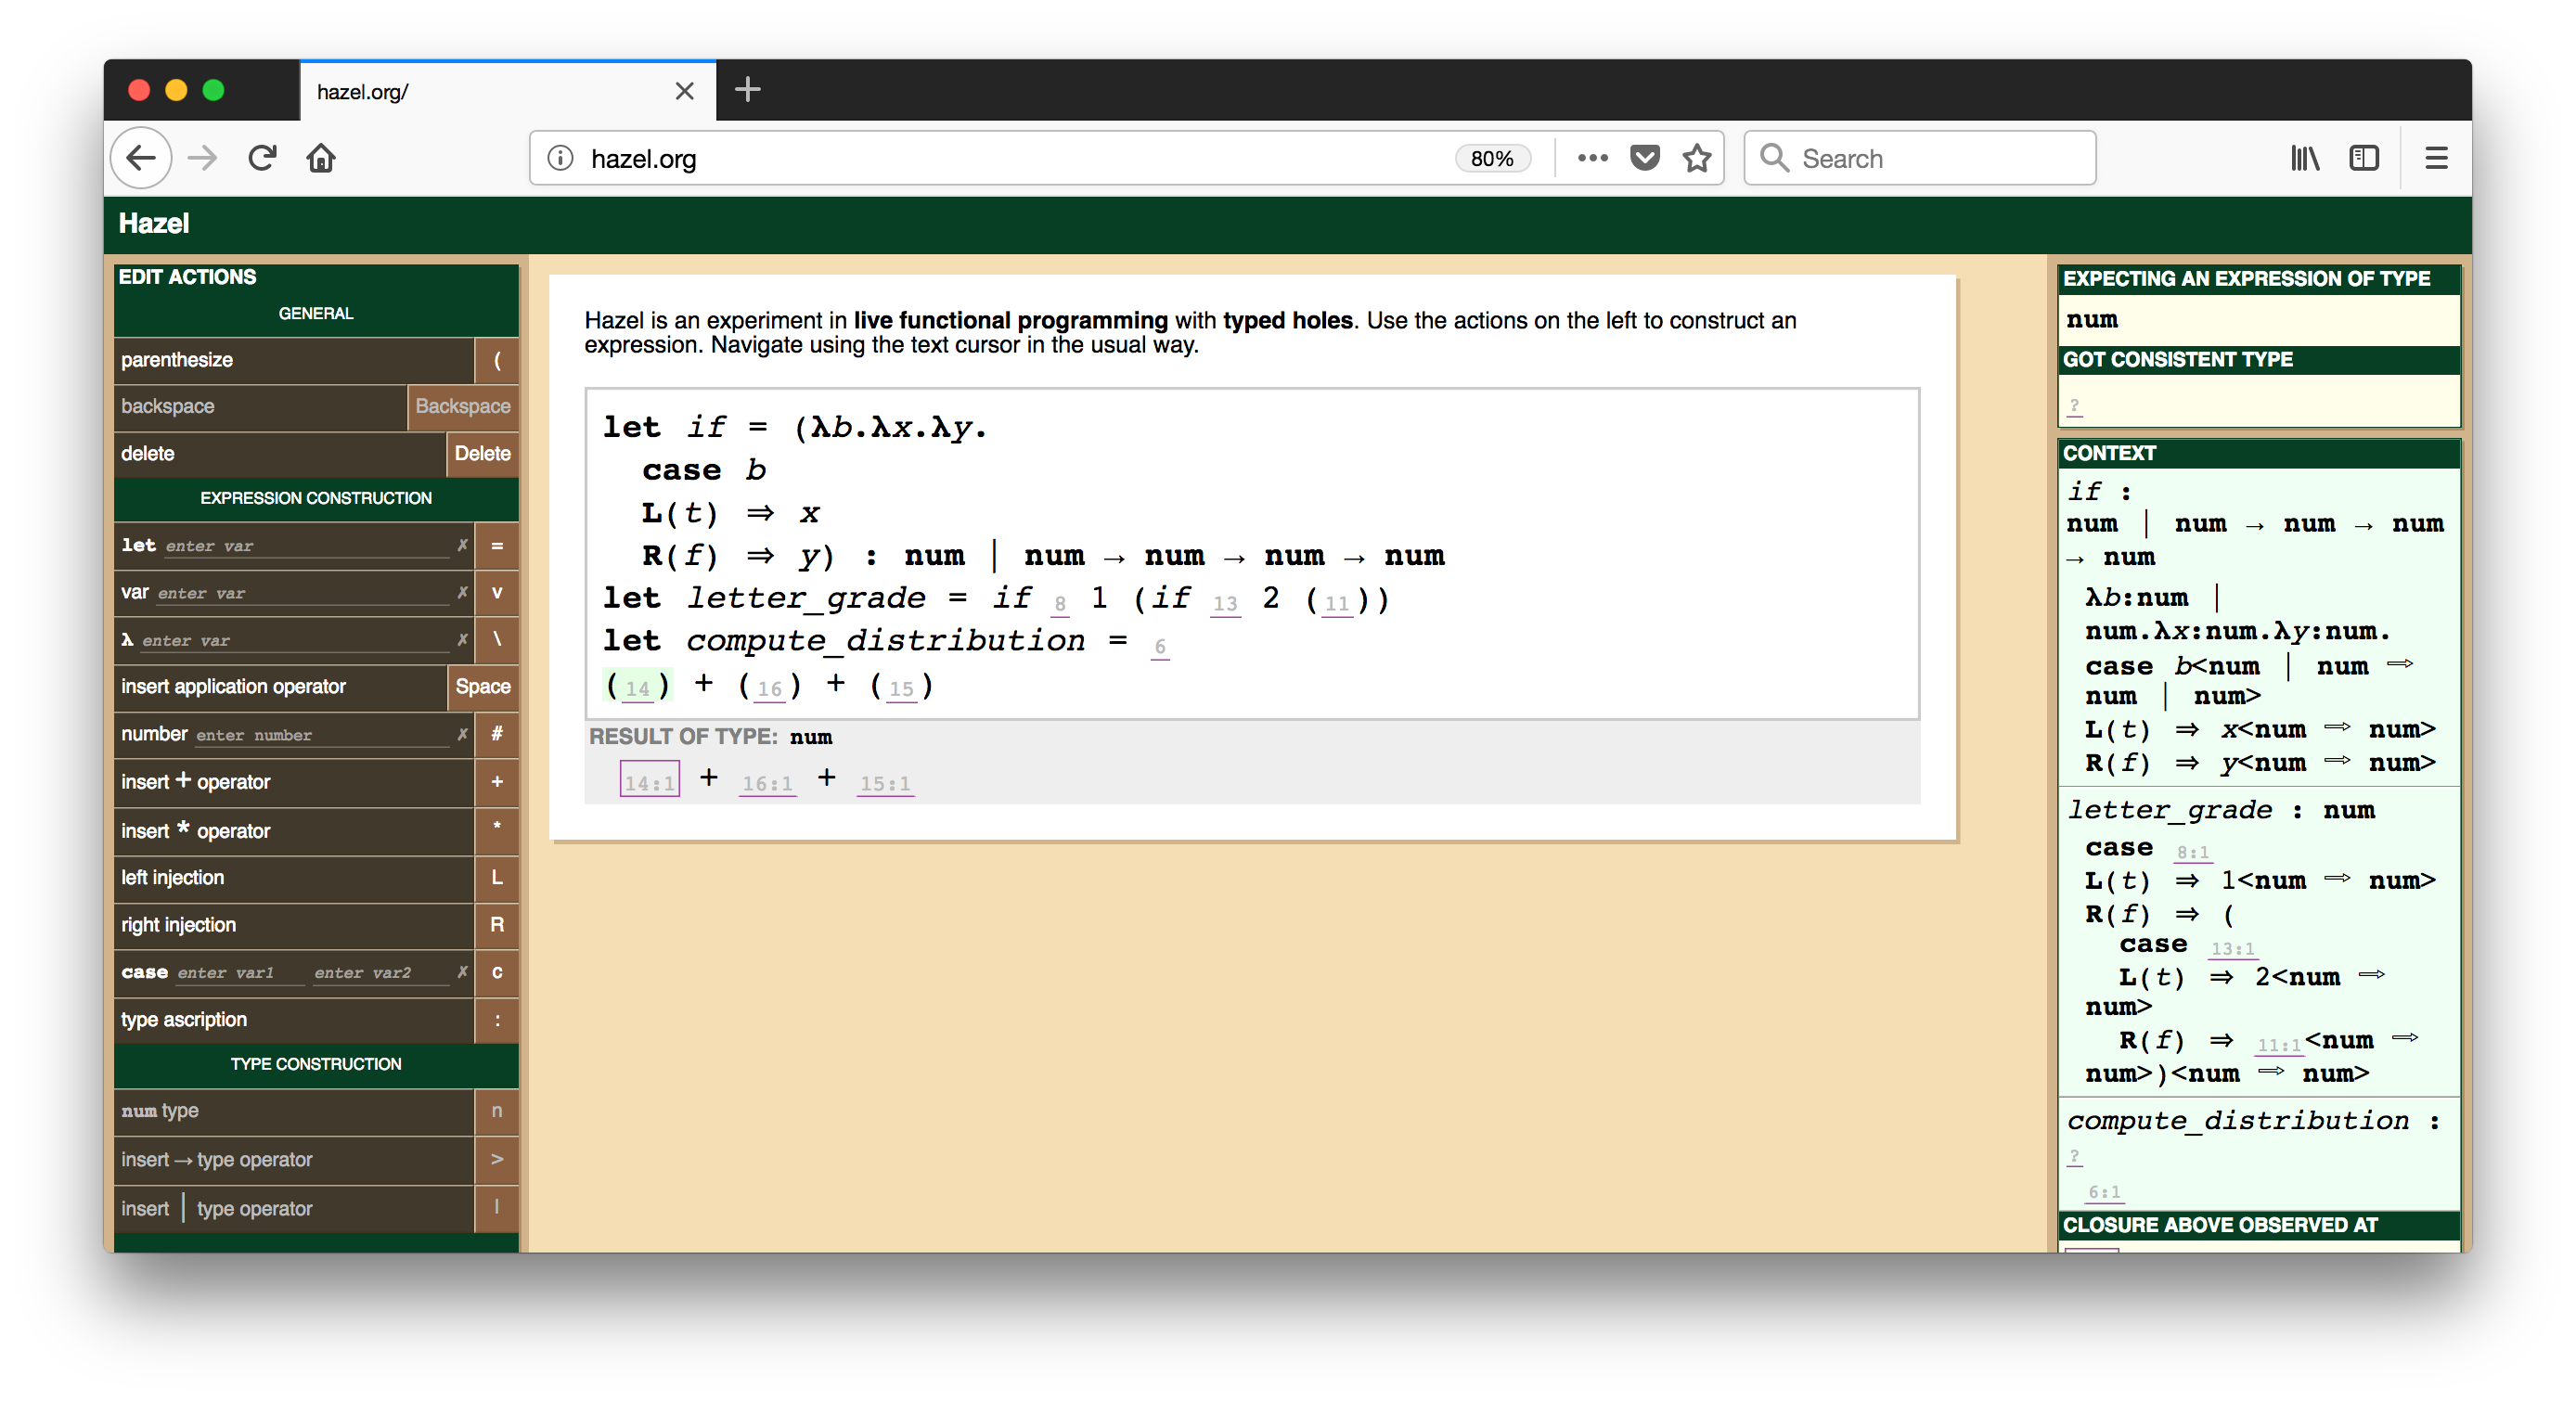
\includegraphics[scale=0.27]{images/hazel-placeholder-1b.png}

\caption{Hazel mockup for Example 1b.}
\label{fig:grades-example-b}
\end{figure}


\overviewExample{1b}{Assigning Letter Grades}
%
The teacher's next task is to map the weighted averages to the letter grades A
through F (we consider only ``whole'' letter grades, for simplicity).
%
The \li{grade_cutoffs} record type, shown at the top of
\autoref{fig:grades-example-b}, describes the minimum cutoff for each of
these six possible grades.
%
Initially, each value in the \li{cutoffs} record is a hole.

%
%% initially all holes, because it will be different year-to-year based on the %
%data, differences in course difficulty, and to satisfy fairness criteria.
%
Before starting to fill in the cutoff values, the teacher jumps ahead to write a
function \li{letter_grade} that will make the connection between \li{cutoffs}
and \li{weighted_averages}.
%
Because she intends to look at the data to help select the cutoff values, the
teacher sorts the \li{weighted_averages} (on line \rkc{XXX}) and then maps
them to \li{letter_grades} (on line \rkc{XXX}).

When \Hazel{} runs this program, the guard of the outermost conditional
(\li{n >= cutoffs.a} on line \rkc{XXX}), is indeterminate because \li{cutoffs.a}
is.
%
Therefore, each of the indeterminate expressions in \li{letter_grades} is the
entire expression body, albeit with different bindings for \li{n}.
%
Displaying such ``large'' indeterminate expressions can quickly consume all
available screen space, overwhelming the user with too much information.
%
\autoref{fig:XXX} shows how \Hazel{} renders large indeterminate
expressions (\ie{}~anything other than ``small'' indeterminate value (a constant
or hole) or list of small values) simply as \li{..} to save space.
%
Hovering over this abbreviation (\rkc{???}) displays the full
indeterminate expression---as well as the evaluation environment that surrounds
it---as a tooltip.
%
\autoref{sec:discussion} discusses this and other user interface concerns when
trying to display useful live feedback without overwhelming the user.
%
These usability factors are beyond the scope of our work, which is to define
semantic foundations on which such user interfaces can be built.

To start deciding \li{cutoffs}, the teacher clicks the \li{weighted_averages}
expression, and views the results panel to see the data sorted in descending
order.
%
The result shows a natural gap between \li{92.2} and \li{89.5}.
%
So, she chooses to use \li{92.0} as the cutoff for A, replacing hole \li{XXX} on
line \rkc{XXX} with that numeric value.
%
Resuming the computation from before, \Hazel{} resolves the conditional
expressions for the first \rkc{XXX} indeterminate expressions, because each of
those \li{n} values was greater than \li{cutoffs.a}.
%
The remaining \rkc{XXX} expressions also proceeded to evaluate the first guard,
and are now indeterminate at the guard for the second conditional.

Before assigning subsequent cutoff values, the teacher would like to get a sense
of whether this first choice is a good one.
%
She jumps ahead to to write a function (\li{compute_distribution} on lines
rkc{XXX}-\rkc{XXX}) that computes the distribution of letter grades based
on \verb+cutoffs+..
%
Running \li{compute_distribution} shows that the percentage of As is
\rkc{XXX\%}, which is smaller than what the teacher would like;
the remaining percentages are all indeterminate.
%
Returning to the value of \li{sorted_data}, she sees a cluster around \li{89.0}
and then another gap between \li{88.2} and {85.5}.
%
So, the teacher adjusts \li{cutoffs.a} to be \li{88.0}.
%
Because this edit is not just filling a hole expression, \Hazel{} discards the
previous execution state and reevaluates the entire program.
%
Existing techniques for incremental computation~\cite{XXX,XXX}, however, could
be applied to seek opportunities for reuse even when non-hole expressions are
modified.
%
Because the focus of work is on the novel implications of running programs with
holes, our calculus and implementation supports caching ``edit-and-resume'' only
for the novel situation in which evaluation proceeds around holes.
%
After re-evaluation, the percentage of As becomes \rkc{XXX\%}, which better
matches the teacher's intention.

In this fashion, the teacher continues down the list of sorted averages,
determining appropriate values for each cutoff.
%
Whenever the teacher is only filling in the ``next'' cutoff, the computation
from before can simply be resumed.
%
Overall, throughout the workflow described in these two examples, the programmer
can continue to evaluate the program, and receive meaningful feedback, while
going back and forth between different pieces under development.
